% Womelsdorf Lab burst library user guide - Algorithms
% Written by Christopher Thomas.

\chapter{Segmentation and Parametric Representation}
\label{sect-math}

%
%
%
\section{Segmentation -- Detecting Burst Events}
\label{sect-math-segment}

``Segmentation'' is the process of deciding which portions of an input
signal contain oscillatory bursts. Historically, this has usually been done
by performing a Hilbert transform to get an analytic signal with known
magnitude and phase, and looking for magnitude excursions above some
threshold (usually $3\sigma$ with respect to the mean magnitude across all
parts of the waveform and all trials). Many variants of this approach exist,
and several other approaches have been used, but these are beyond the scope
of this document.

The wlBurst library provides an implementation of magnitude-threshold
detection, using the algorithm illustrated in Figure \ref{fig-math-algmag}.
Rather than using a fixed threshold, this implementation uses a
low-pass-filtered version of the magnitude as its ``DC'' level, and looks
for magnitude excursions with respect to that (comparing to a local rather
than global mean). The intention is that this is less sensitive to drift
in signal properties.

A typical event segmented by magnitude thresholding is shown in Figure
\ref{fig-math-evmag}. Notice that the analytic magnitude (orange envelope
in the top pane) is only well-behaved for the band-pass-filtered signal.

\figdef{\begin{center}
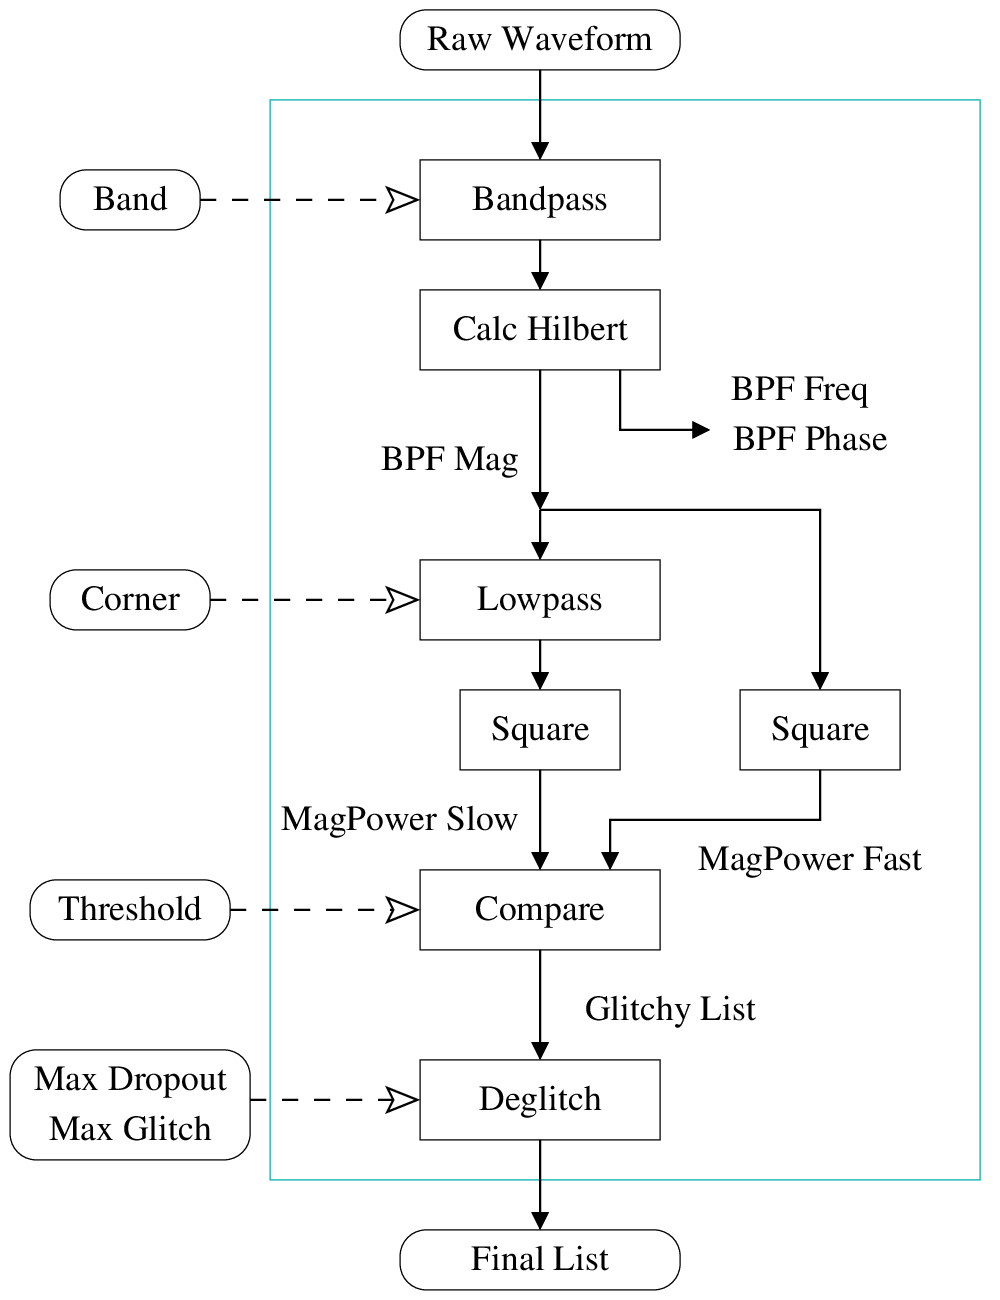
\includegraphics[width=6in]{figs/alg-detmag-v1.png}\end{center}}
{Segmentation by Magnitude Thresholding}
{fig-math-algmag}

\figdef{\begin{center}
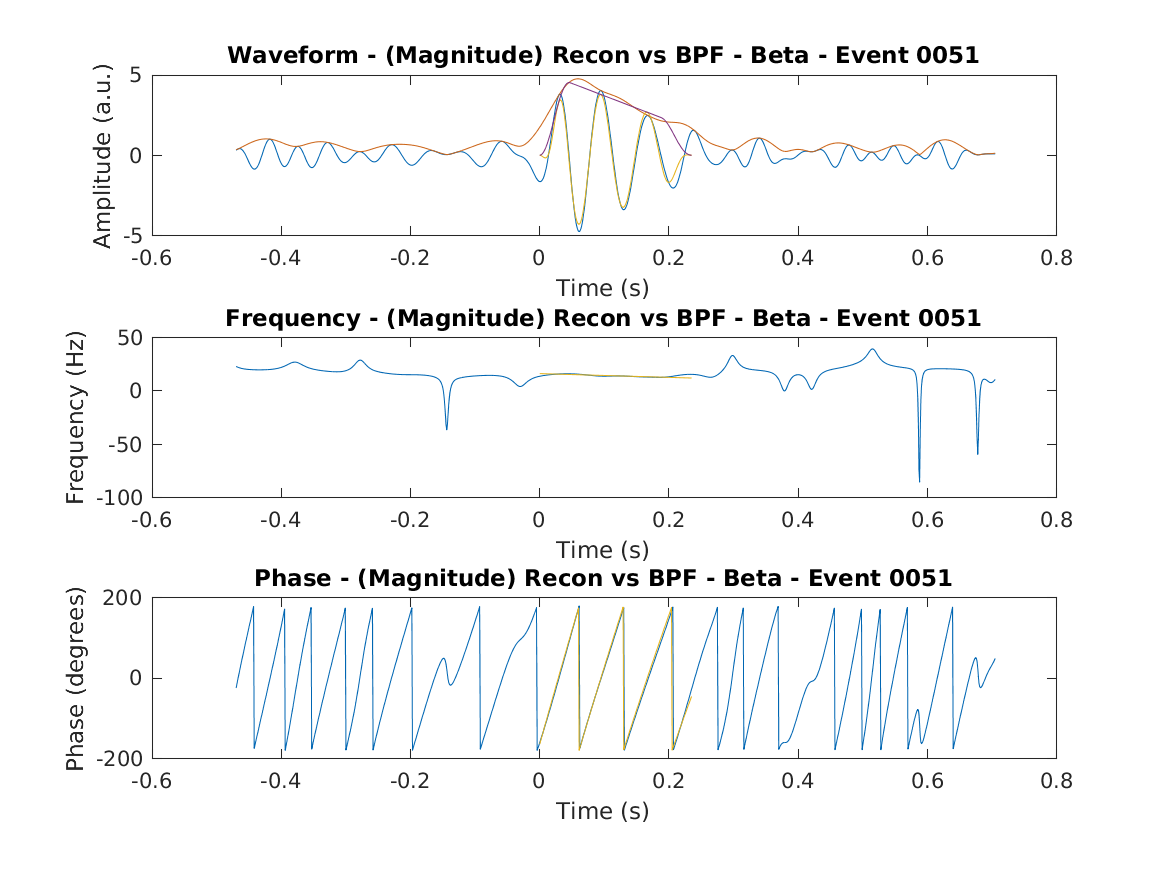
\includegraphics[height=3.5in]{plots/multi-evmag-be-vsbpf-0051.png} \\
Bandpass \\
\vspace{2\baselineskip}
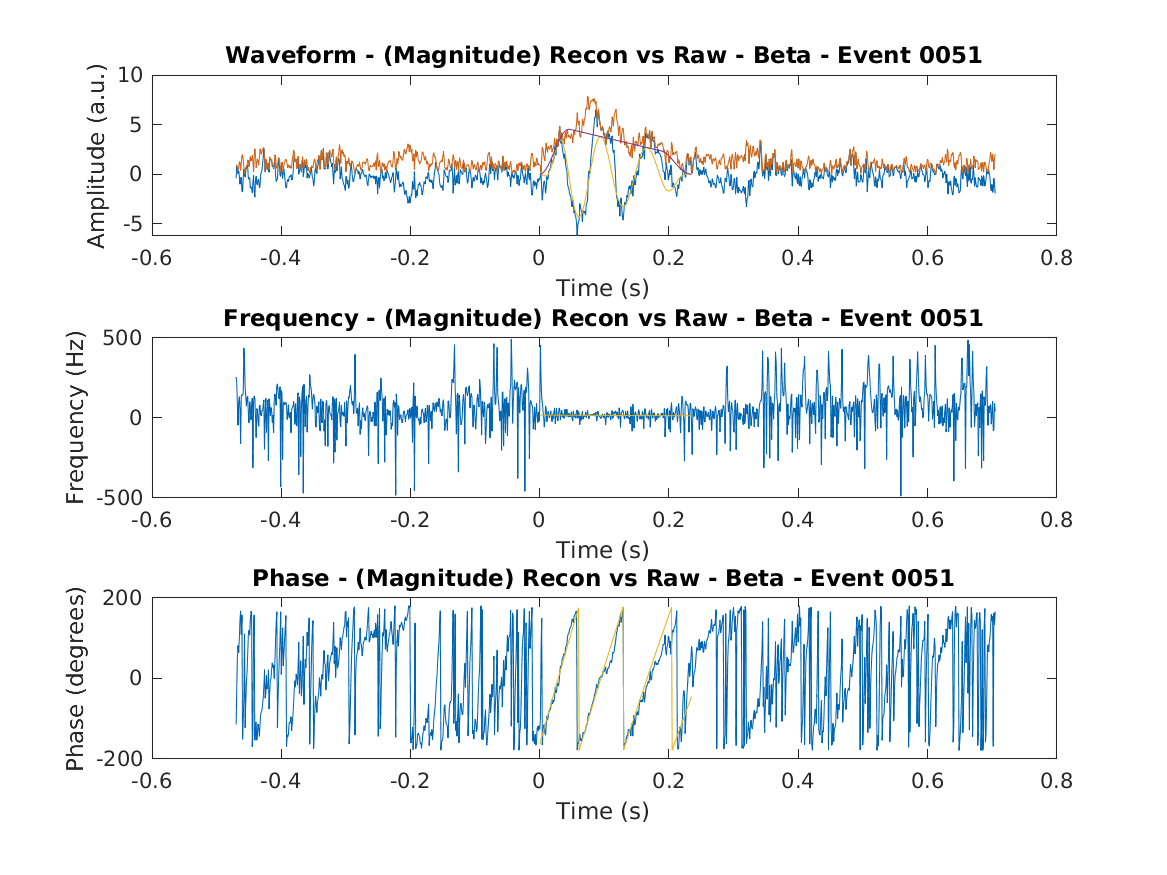
\includegraphics[height=3.5in]{plots/multi-evmag-be-vsraw-0051.png} \\
Wideband
\end{center}}
{Typical event segmented by magnitude thresholding.}
{fig-math-evmag}

\FloatBarrier

In addition to magnitude-threshold event detection, the wlBurst library
provides an implementation of ``frequency-stability'' event detection. This
algorithm looks at the frequency of the analytic signal (middle panes in
Figure \ref{fig-math-evmag}. The analytic frequency is defined as the
derivative of the phase of the analytic signal (which is provided directly
by the Hilbert transform).

During oscillation events, the frequency is expected to be well-defined
(staying within a narrow range with few or no excursions). Outside of
oscillation events, when the neural signal is not oscillating with a
well-defined frequency, excursions in analytic frequency are expected to
occur. These two situations are difficult to distinguish in the Hilbert
transform of the band-pass-filtered waveform, but are visually apparent
in the Hilbert transform of the wideband signal.

To perform automated segmentation, high-frequency noise with known
properties is added to the band-pass-filtered signal. The Hilbert transform
of this ``noisy'' signal is computed, and the variance of the resulting
analytic frequency signal is measured. This algorithm is illustrated
in Figure \ref{fig-math-algfreq}.

A typical event segmented by frequency stability detection is shown in
Figure \ref{fig-math-evfreq}. Notice that the wideband signal shows
out-of-band events, and that the band-pass-filtered signal with added
noise shows only in-band events and has more consistenly different variance
in the frequency signal between event and non-event regions. The ``noisy''
signal is only used for detection - parameter extraction uses the clean
band-pass-filtered signal.

\figdef{\begin{center}
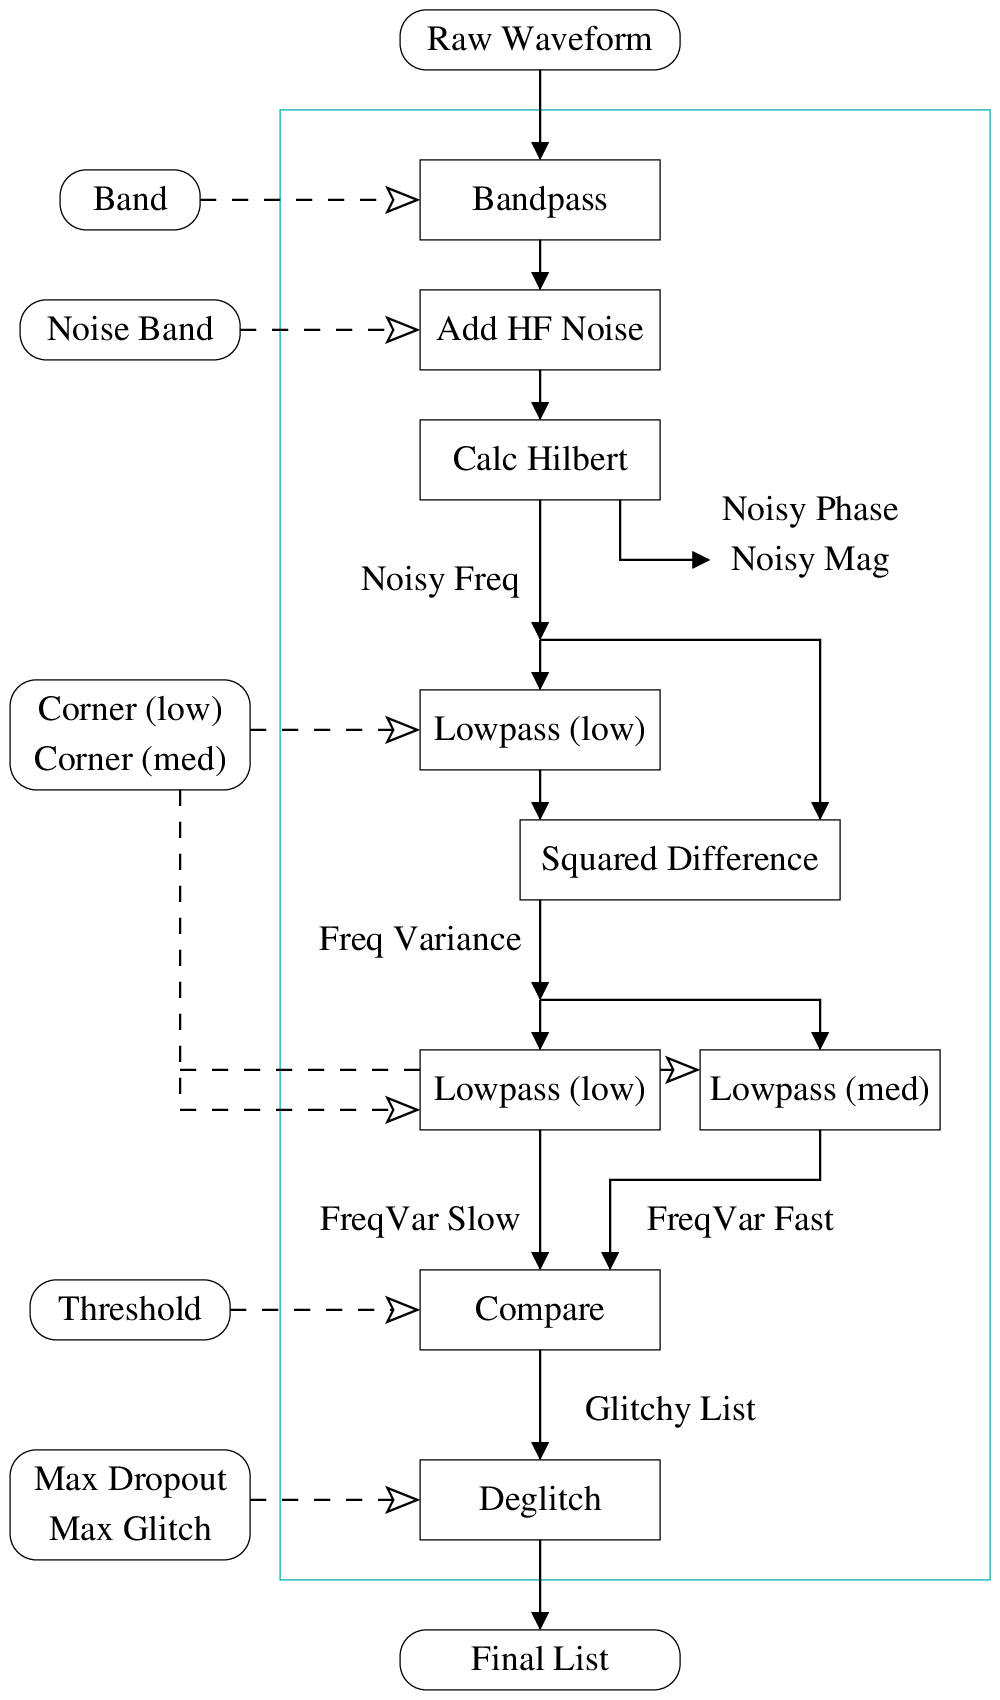
\includegraphics[height=7.5in]{figs/alg-detfreq-v1.png}\end{center}}
{Segmentation by Frequency Stability}
{fig-math-algfreq}

\figdef{\begin{center}
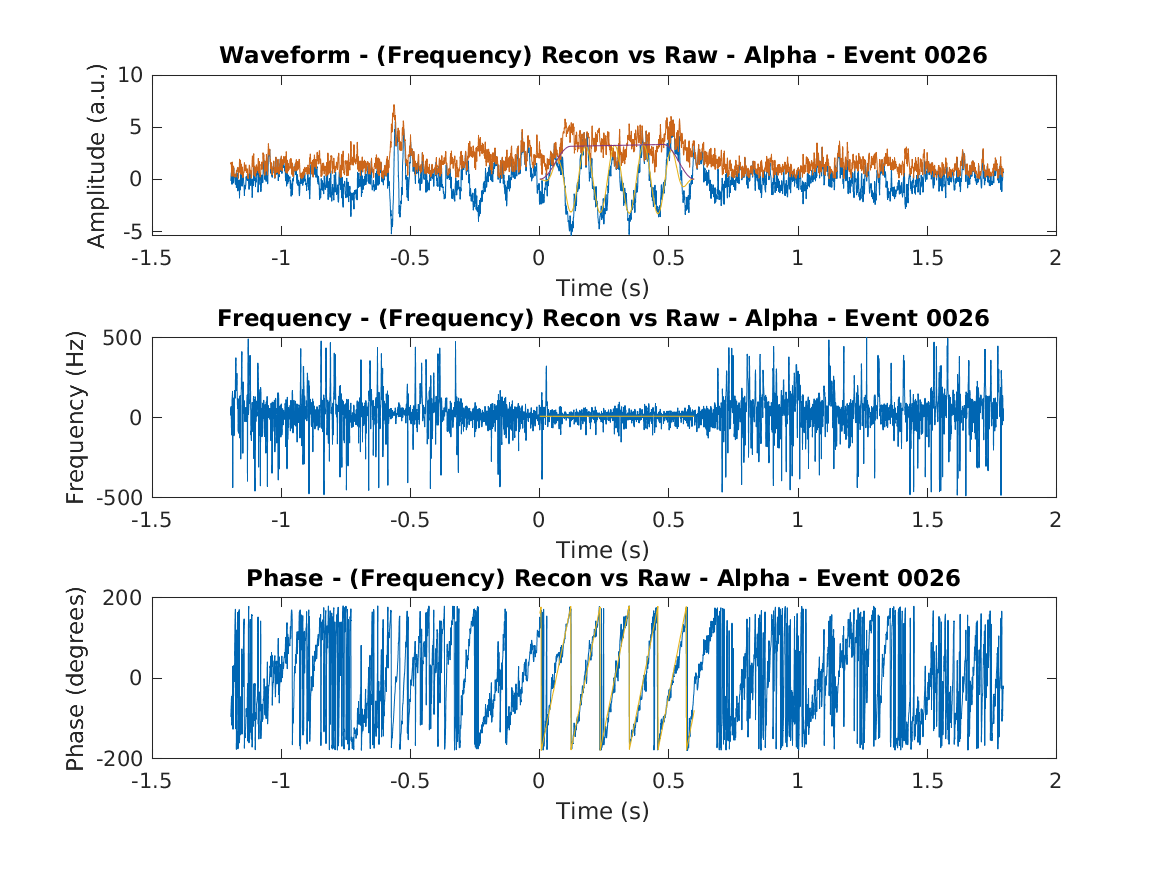
\includegraphics[height=3.5in]{plots/multi-evfreq-al-vsraw-0026.png} \\
Wideband \\
\vspace{2\baselineskip}
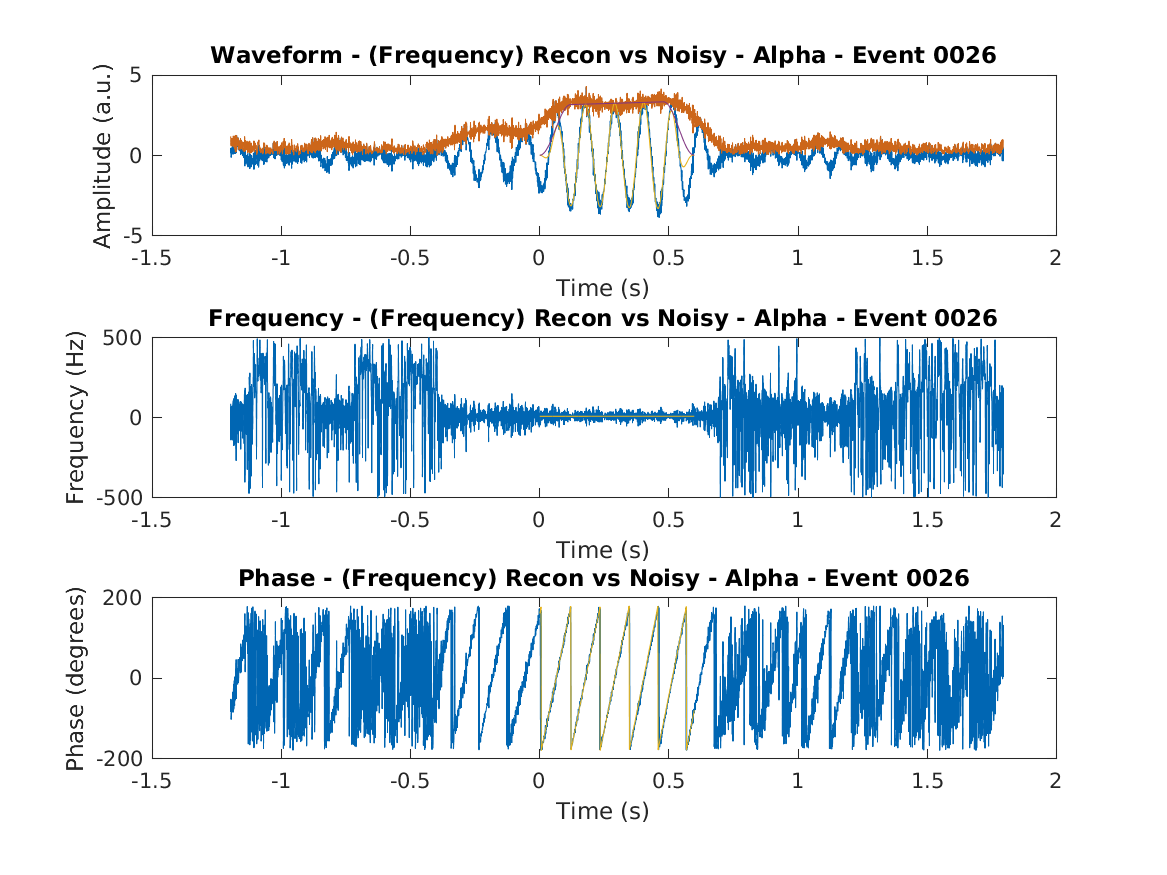
\includegraphics[height=3.5in]{plots/multi-evfreq-al-vsnoisy-0026.png} \\
BPF Plus Noise
\end{center}}
{Typical event segmented by frequency stability.}
{fig-math-evfreq}

\FloatBarrier

%
%
%
\section{Feature Extraction -- Curve-Fitting Oscillatory Bursts}
\label{sect-math-param}

``Feature extraction'' or ``parameter extraction'' is the process of
building a description of a burst event that contains all desired information
about the burst. This is usually done as a separate step after segmentation
(burst detection). The model used to represent oscillatory bursts in the
wlBurst library is shown in Figure \ref{fig-math-params}, and is described
in \texttt{EVENTFORMAT.txt} (as the ``chirpramp'' model). Future versions
of the wlBurst library will explicitly support additional models; for the
time being, custom models may be used provided care is taken to not call
analysis or plotting functions that assume use of the ``chirpramp'' model.

\figdef{\begin{center}
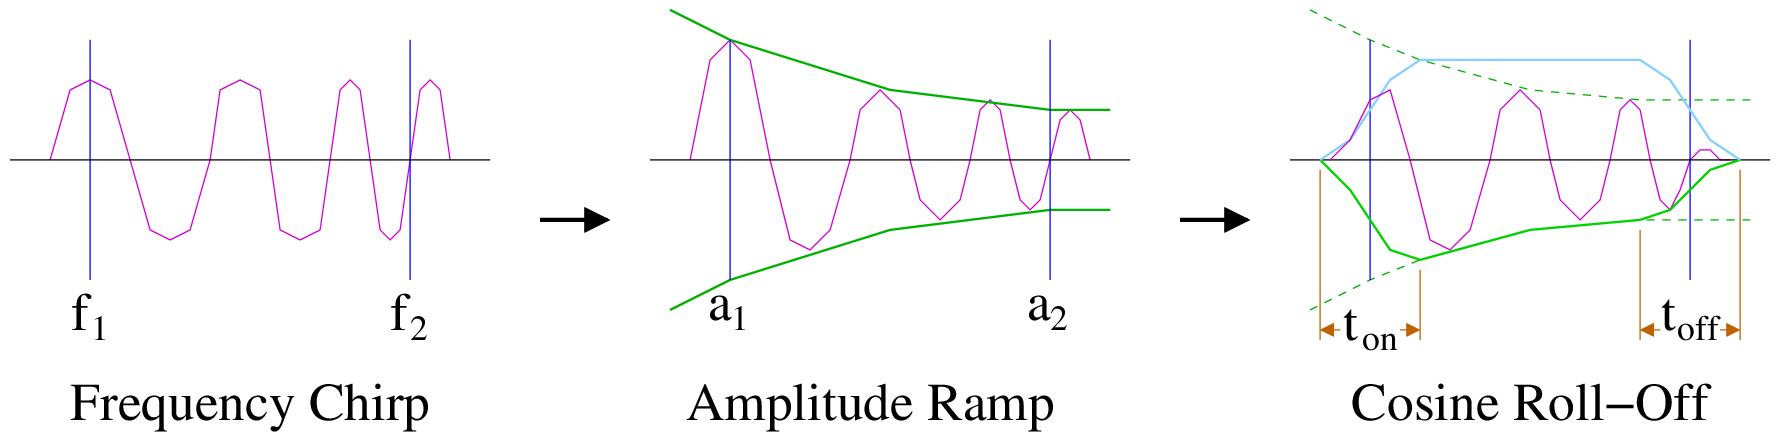
\includegraphics[width=0.9\textwidth]{figs/synth-burst.png}
\end{center}}
{Parametric burst model (``\texttt{chirpramp}'' model).}
{fig-math-params}

``Chirpramp'' model fits are performed through several steps:

\begin{itemize}
%
\item Endpoints of the burst are assumed. These may either be the times
when the detection criterion (absolute magnitude or frequency variance)
crossed its threshold, or where the detection criterion crosses some other
lower threshold (for ``dual'' variants of the magnitude-threshold and
frequency-stability detection algorithms).
%
\item The magnitude envelope is curve-fit. This involves choosing roll-on
and roll-off times, and performing exponential and linear fits to the
analytic magnitude and choosing the best match. Choosing roll-on and roll-off
times may be done via a grid search (fast but less accurate) or by simulated
annealing (slow but more accurate).
%
\item The frequency and phase are curve-fit. This involves performing
exponential and linear fits to the analytic frequency and choosing the best
match, followed by testing possible starting phases and choosing the one that
best matches modeled burst phase and the analytic phase across the duration
of the burst.
%
\item Optionally, a simulated annealing algorithm may perturb all components
of the parametric burst to try to better match the input waveform. This is
slow but slightly improves accuracy.
%
\end{itemize}

User-specified segmentation and parameter extraction algorithms may
alternatively be used, per \linebreak
\texttt{SEGCONFIG.txt} and \texttt{PARAMCONFIG.txt}.


%
% This is the end of the file.
